\documentclass[]{book}
\usepackage{lmodern}
\usepackage{amssymb,amsmath}
\usepackage{ifxetex,ifluatex}
\usepackage{fixltx2e} % provides \textsubscript
\ifnum 0\ifxetex 1\fi\ifluatex 1\fi=0 % if pdftex
  \usepackage[T1]{fontenc}
  \usepackage[utf8]{inputenc}
\else % if luatex or xelatex
  \ifxetex
    \usepackage{mathspec}
  \else
    \usepackage{fontspec}
  \fi
  \defaultfontfeatures{Ligatures=TeX,Scale=MatchLowercase}
\fi
% use upquote if available, for straight quotes in verbatim environments
\IfFileExists{upquote.sty}{\usepackage{upquote}}{}
% use microtype if available
\IfFileExists{microtype.sty}{%
\usepackage{microtype}
\UseMicrotypeSet[protrusion]{basicmath} % disable protrusion for tt fonts
}{}
\usepackage[margin=1in]{geometry}
\usepackage{hyperref}
\hypersetup{unicode=true,
            pdftitle={htmlwidgets中文教程},
            pdfauthor={徐静 译},
            pdfborder={0 0 0},
            breaklinks=true}
\urlstyle{same}  % don't use monospace font for urls
\usepackage{natbib}
\bibliographystyle{apalike}
\usepackage{color}
\usepackage{fancyvrb}
\newcommand{\VerbBar}{|}
\newcommand{\VERB}{\Verb[commandchars=\\\{\}]}
\DefineVerbatimEnvironment{Highlighting}{Verbatim}{commandchars=\\\{\}}
% Add ',fontsize=\small' for more characters per line
\usepackage{framed}
\definecolor{shadecolor}{RGB}{248,248,248}
\newenvironment{Shaded}{\begin{snugshade}}{\end{snugshade}}
\newcommand{\KeywordTok}[1]{\textcolor[rgb]{0.13,0.29,0.53}{\textbf{#1}}}
\newcommand{\DataTypeTok}[1]{\textcolor[rgb]{0.13,0.29,0.53}{#1}}
\newcommand{\DecValTok}[1]{\textcolor[rgb]{0.00,0.00,0.81}{#1}}
\newcommand{\BaseNTok}[1]{\textcolor[rgb]{0.00,0.00,0.81}{#1}}
\newcommand{\FloatTok}[1]{\textcolor[rgb]{0.00,0.00,0.81}{#1}}
\newcommand{\ConstantTok}[1]{\textcolor[rgb]{0.00,0.00,0.00}{#1}}
\newcommand{\CharTok}[1]{\textcolor[rgb]{0.31,0.60,0.02}{#1}}
\newcommand{\SpecialCharTok}[1]{\textcolor[rgb]{0.00,0.00,0.00}{#1}}
\newcommand{\StringTok}[1]{\textcolor[rgb]{0.31,0.60,0.02}{#1}}
\newcommand{\VerbatimStringTok}[1]{\textcolor[rgb]{0.31,0.60,0.02}{#1}}
\newcommand{\SpecialStringTok}[1]{\textcolor[rgb]{0.31,0.60,0.02}{#1}}
\newcommand{\ImportTok}[1]{#1}
\newcommand{\CommentTok}[1]{\textcolor[rgb]{0.56,0.35,0.01}{\textit{#1}}}
\newcommand{\DocumentationTok}[1]{\textcolor[rgb]{0.56,0.35,0.01}{\textbf{\textit{#1}}}}
\newcommand{\AnnotationTok}[1]{\textcolor[rgb]{0.56,0.35,0.01}{\textbf{\textit{#1}}}}
\newcommand{\CommentVarTok}[1]{\textcolor[rgb]{0.56,0.35,0.01}{\textbf{\textit{#1}}}}
\newcommand{\OtherTok}[1]{\textcolor[rgb]{0.56,0.35,0.01}{#1}}
\newcommand{\FunctionTok}[1]{\textcolor[rgb]{0.00,0.00,0.00}{#1}}
\newcommand{\VariableTok}[1]{\textcolor[rgb]{0.00,0.00,0.00}{#1}}
\newcommand{\ControlFlowTok}[1]{\textcolor[rgb]{0.13,0.29,0.53}{\textbf{#1}}}
\newcommand{\OperatorTok}[1]{\textcolor[rgb]{0.81,0.36,0.00}{\textbf{#1}}}
\newcommand{\BuiltInTok}[1]{#1}
\newcommand{\ExtensionTok}[1]{#1}
\newcommand{\PreprocessorTok}[1]{\textcolor[rgb]{0.56,0.35,0.01}{\textit{#1}}}
\newcommand{\AttributeTok}[1]{\textcolor[rgb]{0.77,0.63,0.00}{#1}}
\newcommand{\RegionMarkerTok}[1]{#1}
\newcommand{\InformationTok}[1]{\textcolor[rgb]{0.56,0.35,0.01}{\textbf{\textit{#1}}}}
\newcommand{\WarningTok}[1]{\textcolor[rgb]{0.56,0.35,0.01}{\textbf{\textit{#1}}}}
\newcommand{\AlertTok}[1]{\textcolor[rgb]{0.94,0.16,0.16}{#1}}
\newcommand{\ErrorTok}[1]{\textcolor[rgb]{0.64,0.00,0.00}{\textbf{#1}}}
\newcommand{\NormalTok}[1]{#1}
\usepackage{longtable,booktabs}
\usepackage{graphicx,grffile}
\makeatletter
\def\maxwidth{\ifdim\Gin@nat@width>\linewidth\linewidth\else\Gin@nat@width\fi}
\def\maxheight{\ifdim\Gin@nat@height>\textheight\textheight\else\Gin@nat@height\fi}
\makeatother
% Scale images if necessary, so that they will not overflow the page
% margins by default, and it is still possible to overwrite the defaults
% using explicit options in \includegraphics[width, height, ...]{}
\setkeys{Gin}{width=\maxwidth,height=\maxheight,keepaspectratio}
\IfFileExists{parskip.sty}{%
\usepackage{parskip}
}{% else
\setlength{\parindent}{0pt}
\setlength{\parskip}{6pt plus 2pt minus 1pt}
}
\setlength{\emergencystretch}{3em}  % prevent overfull lines
\providecommand{\tightlist}{%
  \setlength{\itemsep}{0pt}\setlength{\parskip}{0pt}}
\setcounter{secnumdepth}{5}
% Redefines (sub)paragraphs to behave more like sections
\ifx\paragraph\undefined\else
\let\oldparagraph\paragraph
\renewcommand{\paragraph}[1]{\oldparagraph{#1}\mbox{}}
\fi
\ifx\subparagraph\undefined\else
\let\oldsubparagraph\subparagraph
\renewcommand{\subparagraph}[1]{\oldsubparagraph{#1}\mbox{}}
\fi

%%% Use protect on footnotes to avoid problems with footnotes in titles
\let\rmarkdownfootnote\footnote%
\def\footnote{\protect\rmarkdownfootnote}

%%% Change title format to be more compact
\usepackage{titling}

% Create subtitle command for use in maketitle
\newcommand{\subtitle}[1]{
  \posttitle{
    \begin{center}\large#1\end{center}
    }
}

\setlength{\droptitle}{-2em}

  \title{htmlwidgets中文教程}
    \pretitle{\vspace{\droptitle}\centering\huge}
  \posttitle{\par}
    \author{徐静 译}
    \preauthor{\centering\large\emph}
  \postauthor{\par}
      \predate{\centering\large\emph}
  \postdate{\par}
    \date{2018-07-02}

\usepackage{booktabs}

\usepackage{amsthm}
\newtheorem{theorem}{Theorem}[chapter]
\newtheorem{lemma}{Lemma}[chapter]
\theoremstyle{definition}
\newtheorem{definition}{Definition}[chapter]
\newtheorem{corollary}{Corollary}[chapter]
\newtheorem{proposition}{Proposition}[chapter]
\theoremstyle{definition}
\newtheorem{example}{Example}[chapter]
\theoremstyle{definition}
\newtheorem{exercise}{Exercise}[chapter]
\theoremstyle{remark}
\newtheorem*{remark}{Remark}
\newtheorem*{solution}{Solution}
\begin{document}
\maketitle

{
\setcounter{tocdepth}{1}
\tableofcontents
}
\chapter*{声明}
\addcontentsline{toc}{chapter}{声明}

htmlwidgets是R语言中非常有划时代意义的包,因为有了htmlwidgets使得R语言在交互可视化和Web编程有了实质性的进步。htmlwidgets目前没有中文说明文档和教程,该文档是对官方文档的详细翻译,译者水平有限,网读者留言指正。

\chapter*{序言}
\addcontentsline{toc}{chapter}{序言}

htmlwidgets,一个用来创建HTML控件的包,可以运行在R命令行, R Markdown,
Shiny。

\begin{verbatim}
Type Package
Title HTML Widgets for R
Version 1.2
Description A framework for creating HTML widgets that render in various
contexts including the R console, 'R Markdown' documents, and 'Shiny'
web applications.
License MIT + file LICENSE
VignetteBuilder knitr
Imports grDevices, htmltools (>= 0.3), jsonlite (>= 0.9.16), yaml
Suggests knitr (>= 1.8)
Enhances shiny (>= 1.0.5)
URL https://github.com/ramnathv/htmlwidgets
BugReports https://github.com/ramnathv/htmlwidgets/issues
RoxygenNote 6.0.1
NeedsCompilation no
Author Ramnath Vaidyanathan [aut, cph],
Yihui Xie [aut],
JJ Allaire [aut, cre],
Joe Cheng [aut],
Kenton Russell [aut, cph],
RStudio [cph]
Maintainer JJ Allaire <jj@rstudio.com>
Repository CRAN
Date/Publication 2018-04-19 12:43:03 UTC
\end{verbatim}

目前针对于htmlwidgets并没有详细的中文教程,译者会持续更新翻译htmlwidgets,并推出更多基于htmlwidgets的R包。

徐静

联信集团

2018-07-02

\chapter*{关于译者}
\addcontentsline{toc}{chapter}{关于译者}

\textbf{徐静:}

硕士研究生,
目前的研究兴趣主要包括:数理统计,统计机器学习,深度学习,网络爬虫,前端可视化,R语言和Python语言的超级粉丝,多个R包和Python模块的作者,现在正逐步向Java迁移。

\chapter{Introduction}\label{htmlwidgetsux7b80ux4ecb}

\section{概况}

\href{https://cran.r-project.org/web/packages/htmlwidgets/index.html}{htmlwidgets}包提供了一个R语言链接Javascript库的框架,HTML控件能够:

\begin{itemize}
\item
  在R命令中做分析比如方便的R作图
\item
  和R Markdown结合在一起
\item
  和shiny结合在一起
\item
  保存为独立的网页,通过电子邮件,Dropbox等ad-oc共享。
\end{itemize}

通过醉熏一小部分易于尊寻的约定,可以创建非常小的代码和HTML小部件,所有空间包含如下部分:

\begin{enumerate}
\def\labelenumi{\arabic{enumi}.}
\item
  \emph{Dependencies}: 这些事空间用到的需要声明的Javascript和CSS
\item
  \emph{R binding}:
  这是终端用户将调用的功能,以向控件提供输入数据,并制定控件应该如何呈现各种选项,这包括在shiny应用程序中使用控件所需要的一些剪短的样板功能。
\item
  \emph{javaScript binding}:
  这是JavaScript代码,把所有的东西粘在一起。将R绑定中收集的数据和选项传递给底层的JavaScript库
\end{enumerate}

已经有非常多的包基于htmlwidgets去完成,包括:

\begin{itemize}
\item
  leaflet -- 交互的地图绘制包
\item
  dygraphs -- 交互时间序列绘图包
\item
  networkD3 -- 基于D3.js的交互网络图可视化
\item
  sparkline -- 小型的内联图
\item
  DT -- 表格可视化
\item
  rthreejs -- 交互3D图
\end{itemize}

包的作者包括:Ramnath Vaidyanathan, Joe Cheng, JJ Allaire, Yihui Xie,
and Kenton Russell等。

HTML控件一般会寄存在一个R包中,并且应该包含他们的依赖关系的所有源代码,例如这里译者写的以个基于htmlwidgets的R包:\href{https://github.com/DataXujing/XuJIngd3plus}{XuJIngd3plus}。这是为了确保依赖的控件的完全可重复的(既不需要联网,也不需要运行服务器),说白了在你R包中,应该包含所有的源码包括你底层调用的JavaScript包或CSS。

\section{简单的开始}

如果你懂R语言和一点JavaScript,创建自己的小部件非常简单,最先要做的就是要安装htmlwidgets,在CRAN上:

\begin{Shaded}
\begin{Highlighting}[]
\KeywordTok{install.packages}\NormalTok{(}\StringTok{'htmlwidgets'}\NormalTok{)}
\end{Highlighting}
\end{Shaded}

你也可以在GitHub上安装开发版本:

\begin{Shaded}
\begin{Highlighting}[]
\NormalTok{devtools}\OperatorTok{::}\KeywordTok{install_github}\NormalTok{(}\StringTok{'ramnathv/htmlwidgets'}\NormalTok{)}
\end{Highlighting}
\end{Shaded}

通过包中自带的说明文档,让你快速的熟悉htmlwidgets并进入开发者状态,包括:

\begin{itemize}
\item
  Introduction to HTML Widgets
\item
  HTML Widget Sizing
\item
  HTML Widgets: Advanced Topics
\end{itemize}

我们会持续把他们翻译成中文,让中国人看起来更爽。

\section{例子(sigma.js)}\label{sigma.js}

首先,我们将通过创建一个控件来封装\href{http://sigmajs.org/}{sigma.js}图形可视化库。当我们完成后,我们可以用来显示\href{https://gephi.org/gexf/format/}{GEXF}(Graph
Exchange XML Format)数据文件的交互可视化,例如:

\begin{Shaded}
\begin{Highlighting}[]
\KeywordTok{library}\NormalTok{(sigma)}
\NormalTok{data <-}\StringTok{ }\KeywordTok{system.file}\NormalTok{(}\StringTok{"examples/ediaspora.gexf.xml"}\NormalTok{, }\DataTypeTok{package =} \StringTok{"sigma"}\NormalTok{)}
\KeywordTok{sigma}\NormalTok{(data)}
\end{Highlighting}
\end{Shaded}

\begin{figure}
\centering
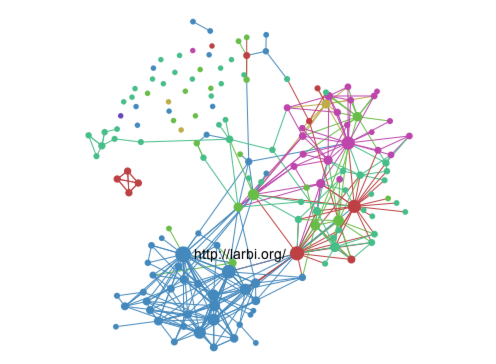
\includegraphics{_bookdown_files/htmlwidgets_cn_files/figure-html/ch1_1.png}
\caption{}
\end{figure}

注意上面的输出仅仅是一个静态图像,你可以做一个按照下文的Demo做一个交互的版本。

创建这种绑定所需的代码非常少。下面我们将一步一步地介绍所有的控件。然后,我们将描述如何创建自己的控件(包括为所有核心组件自动生成基本的脚手架)。

\subsection{Filelayout}\label{filelayout}

\subsection{Dependencies}\label{dependencies}

\subsection{R binding}\label{r-binding}

\subsection{JavaScript bing}\label{javascript-bing}

\subsection{Demo}\label{demo}

\section{创建你自己的widgets}\label{widgets}

\subsection{Requirements}\label{requirements}

\subsection{Scaffolding}\label{scaffolding}

\subsection{Learning more}\label{learning-more}

\subsubsection{Additional articles}\label{additional-articles}

\subsubsection{Examples}\label{examples}

\subsubsection{Questions and issues}\label{questions-and-issues}

\chapter{Advanced}\label{htmlwidgetsux8fdbux9636}

这是进阶

\chapter{Sizing\{\#htmlwidgets Sizing\}}\label{sizinghtmlwidgets-sizing}

Sizing

\chapter{htmlwidgets包的翻译}\label{htmlwidgetsux5305ux7684ux7ffbux8bd1}

htmlwidgets包的翻译

\chapter{总结}

总结

\chapter{参考文献}

\bibliography{book.bib,packages.bib}


\end{document}
